\subsection{Cen�rio Detec��o de Cortes \label{use_case_cortes}}

\begin{figure}[h|top]
 \centering
 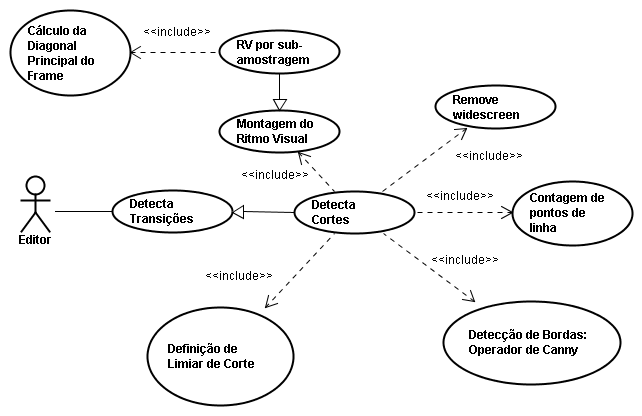
\includegraphics[width=1.0\linewidth]{imagens/use_case_cortes.png}
 \caption{Caso de Uso para cen�rio de detec��o de cortes.}
 \label{img_use_case_cortes}
\end{figure}

A Figura \ref{img_use_case_cortes}, representa o cen�rio espec�fico
de detec��o de cortes.

\subsubsection{Caso de uso: Detecta Cortes \label{use_case_detecta_cortes}}

\textbf{Cen�rio Principal:} Feito o carregamento do v�deo, o
processo de detec��o de transi��es se iniciar� pela detec��o de
cortes.

\subsubsection{Caso de uso: Montagem do Ritmo Visual por sub-amostragem \label{use_case_rv_amostra}}

\textbf{Cen�rio Principal:} Solicitada a detec��o de transi��es de
cortes no v�deo, ser� montado o Ritmo Visual do v�deo atrav�s de
sub-amostragens dos frames do v�deo.

A sub-amostragem � retirada frame a frame de forma seq�encial.

\subsubsection{Caso de uso: C�lculo da diagonal principal do frame \label{use_case_diagonal_principal}}

\textbf{Cen�rio Principal:} Para a montagem do Ritmo Visual, dever�
ser calculada a diagonal principal de todos os frames do v�deo. Tal
diagonal representa a sub-amostragem dos frames.

\subsubsection{Caso de uso: Detec��o de Bordas: Operador Sobel \label{use_case_sobel}}
